\section{实验目的}

\begin{enumerate}
    \item 温习基于 Quartus II 的数字电路设计及仿真方法;
    \item 熟悉 D 触发器的功能及使用方法;
    \item 掌握寄存器组的组成原理。
\end{enumerate}

\section{实验内容}

\begin{enumerate}
    \item 测试 D 触发器的功能;
    \item 设计具有 1 个读端口、1 个写端口的 $4 \times 8$ 位寄存器组,并验证其功能。
\end{enumerate}

\section{实验原理及设计}

\subsection{验证 D 触发器的功能}

D 触发器具有异步置数,异步清除,同步读入,输出等功能。利用仿真文件设定波形,我们就可以通过
修改触发器各个输入端口的信号,检测输出端口的信号来验证 D 触发器的功能。

具体的原理图设计见图 \ref{figure:1.1-design}。

\begin{figure}[h]
    \centering
    \caption{D 触发器功能验证原理图}
    \label{figure:1.1-design}
    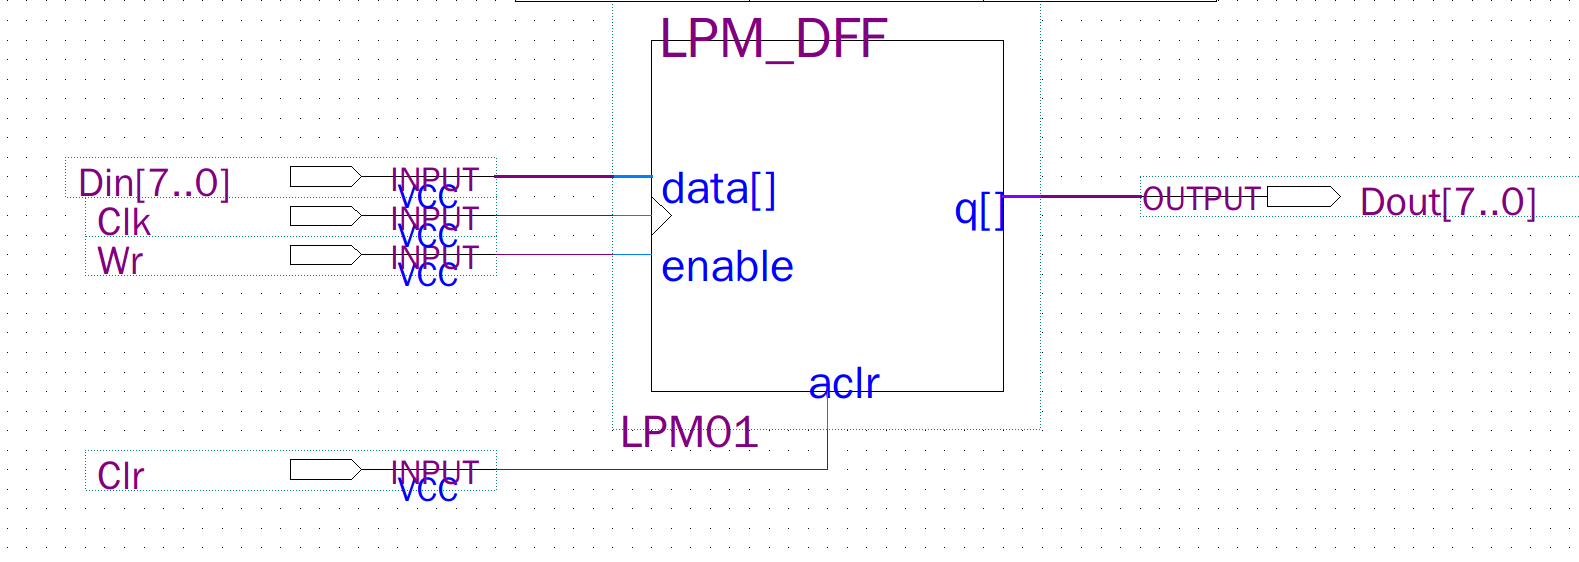
\includegraphics[scale=0.3]{pics/1.1-design.png}
\end{figure}

\subsection{设计寄存器组}

首先需要确定寄存器组的各个端口和功能,具体如表 \ref{table:1.1-func}:

\begin{table}[h]
    \centering
    \caption{寄存器组端口及功能表}
    \label{table:1.1-func}
    \begin{tabular}{|c|c|c|}
        \hline
        端口名称 & 端口宽度 & 端口说明 \\ \hline
        \verb|Clk| & 1 & 时钟信号 \\ \hline
        \verb|Clr| & 1 & 异步置零信号 \\ \hline
        \verb|Wen| & 1 & 写入允许信号,低电平有效 \\ \hline
        \verb|Wa| & 2 & 写入寄存器选择端口,输入目标寄存器的地址,二进制整数 \\ \hline
        \verb|Wd| & 8 & 数据输入端口,输入需要写入的数据 \\ \hline
        \verb|Ra| & 2 & 读出寄存器选择端口,输入目标选择器的地址,二进制整数 \\ \hline
        \verb|Rd| & 8 & 数据输出端口,输出目标寄存器存储的数据 \\ \hline
    \end{tabular}
\end{table}

然后考虑如何实现。

首先,使用 8 位 D 触发器作为各个寄存器。

D 触发器有一个使能端,这可以用于该寄存器是否允许写入。由于输入的寄存器地址 \verb|Wa| 是一个
二进制数,考虑使用译码器来决定导通哪个寄存器。特别的,译码器 74139 有一个译码使能端,这个使能端可以封锁译码器的
输出,因此可以用作整个寄存器组的写入允许端口。

数据输入,时钟信号和置零,则直接将数据输入端口连接至各个寄存器的对应端口即可。

最后,数据输出选择,则可通过一个四选一数据选择器实现。

详细的实现见图 \ref{figure:1.2-design}。

\begin{figure}[h]
    \centering
    \caption{寄存器组设计图}
    \label{figure:1.2-design}
    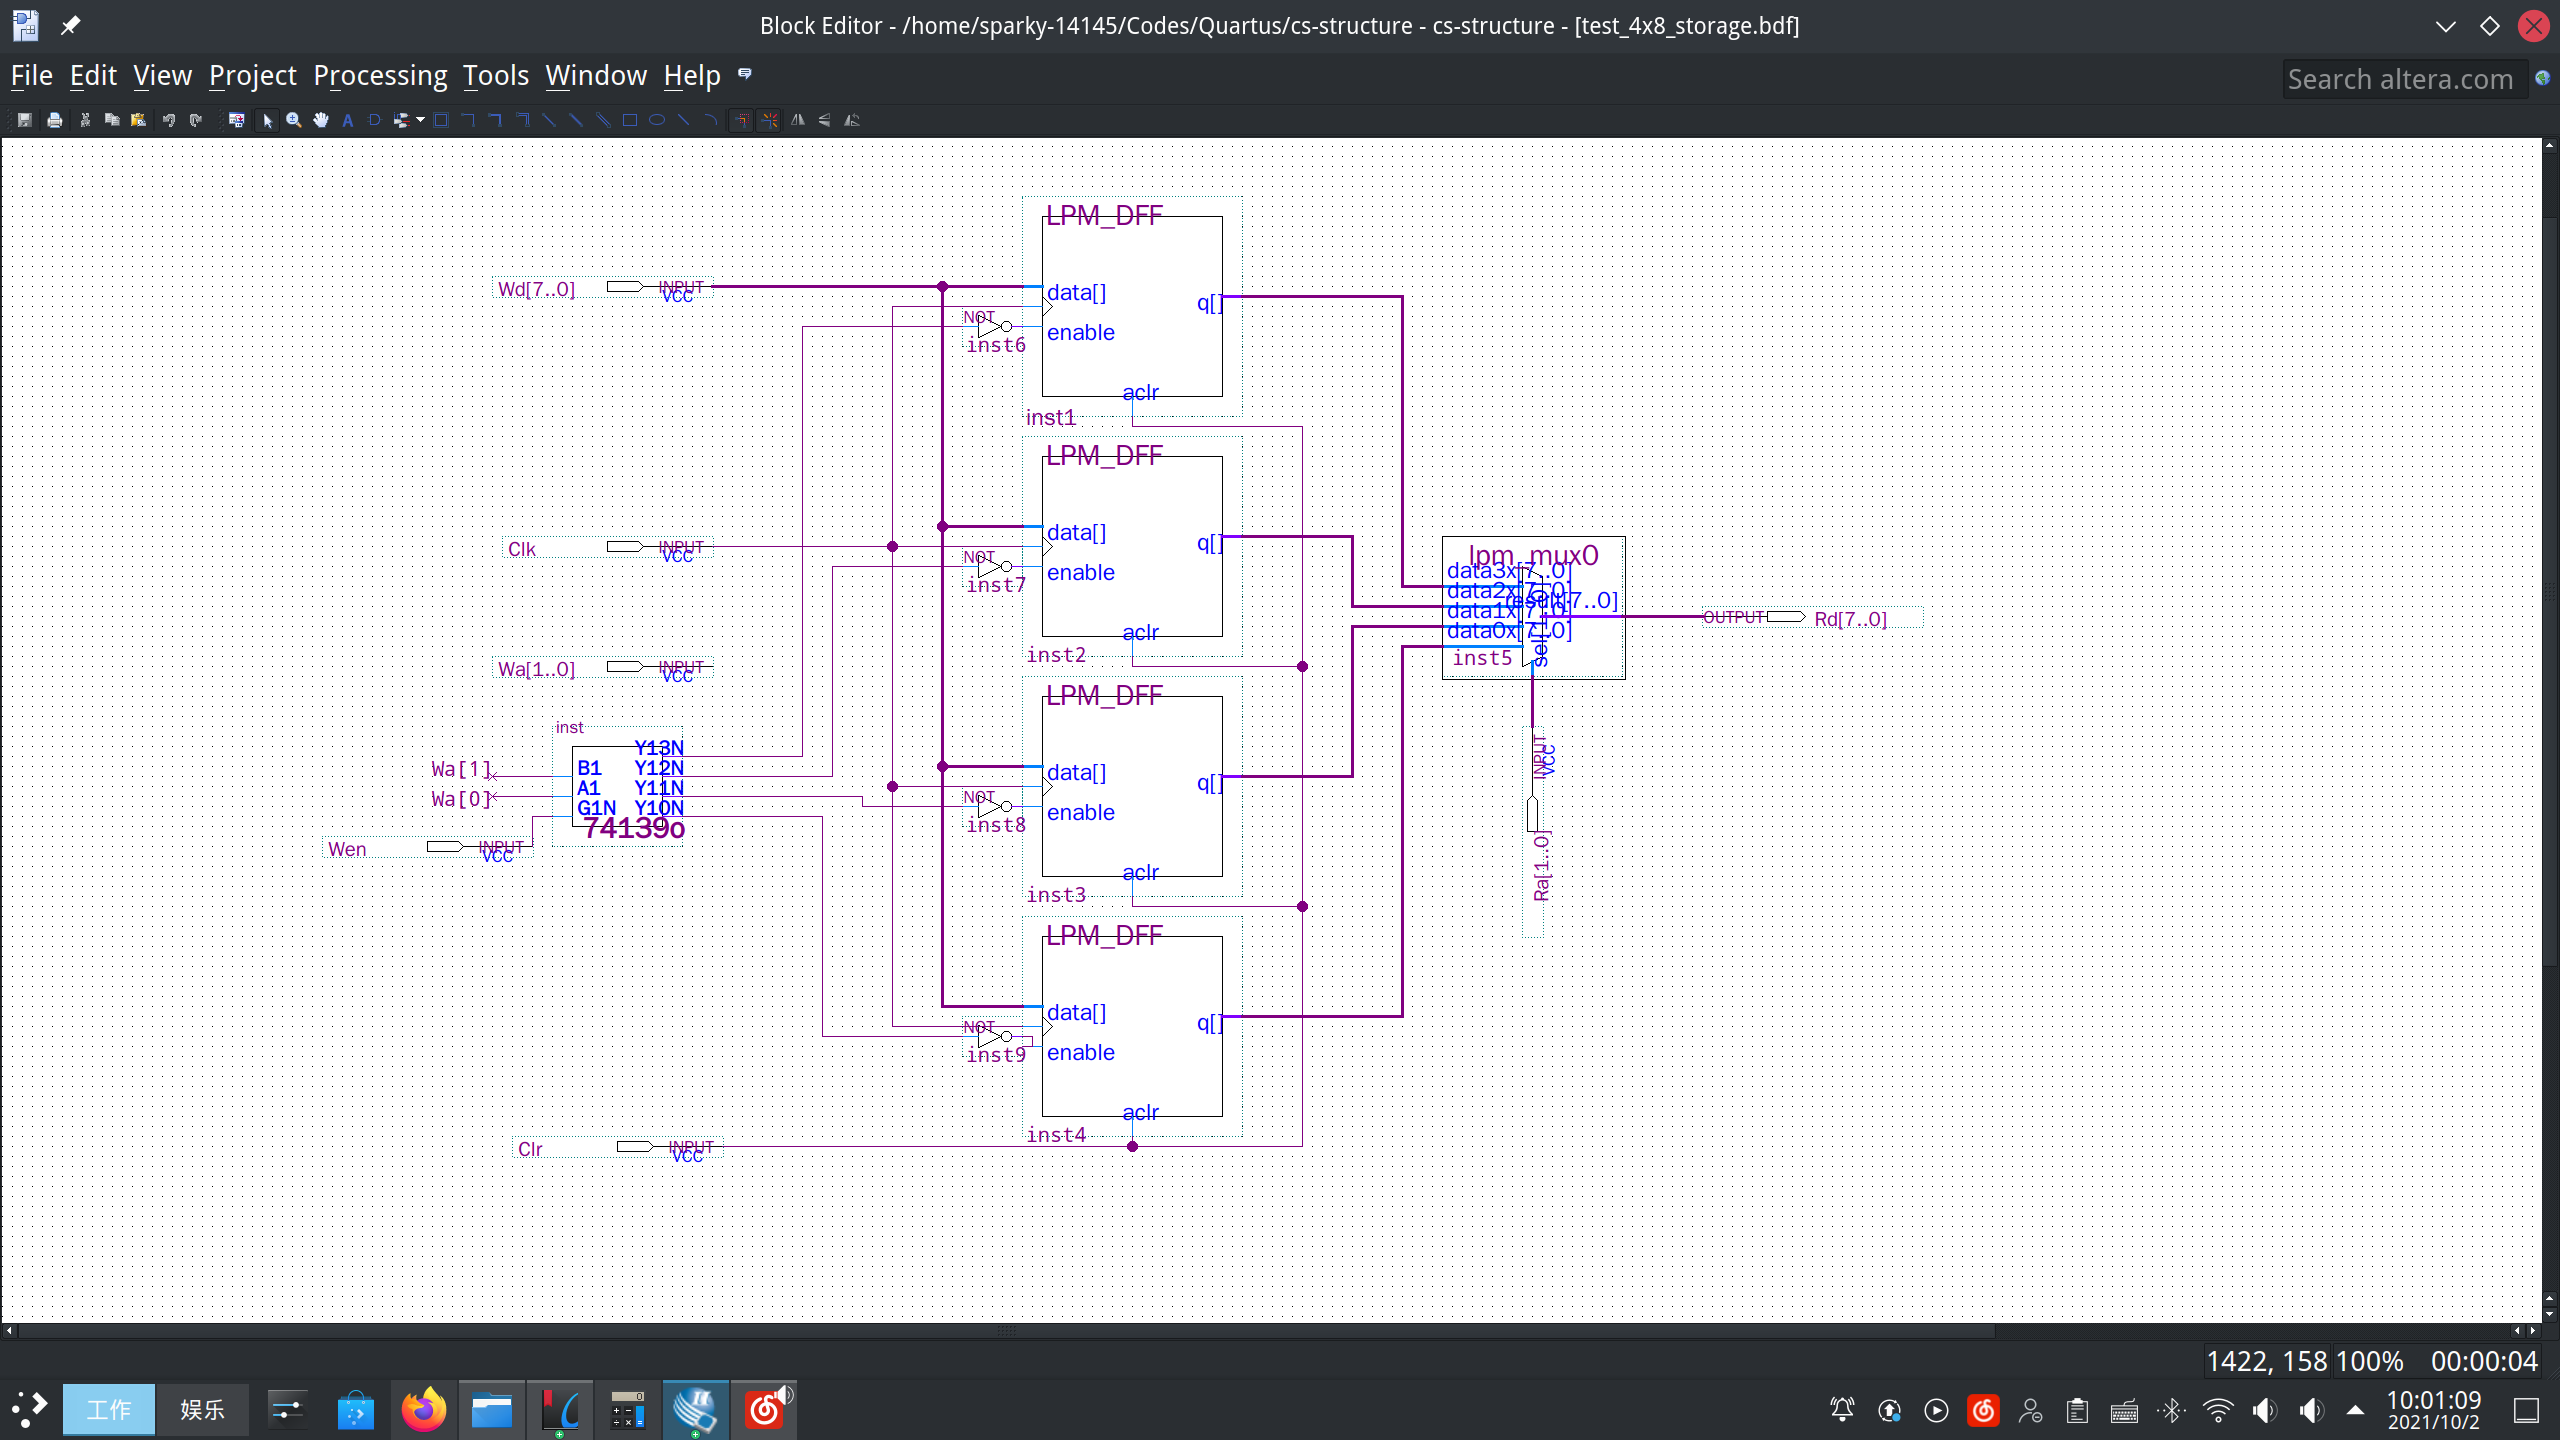
\includegraphics[scale=0.2]{pics/1.2-design.png}
\end{figure}

\section{实验结果}

\subsection{验证 D 触发器的功能}

实验使用的输入波形与结果波形如图 \ref{figure:1.1-result} 所示。

\begin{figure}[h]
    \centering
    \caption{D 触发器功能验证结果}
    \label{figure:1.1-result}
    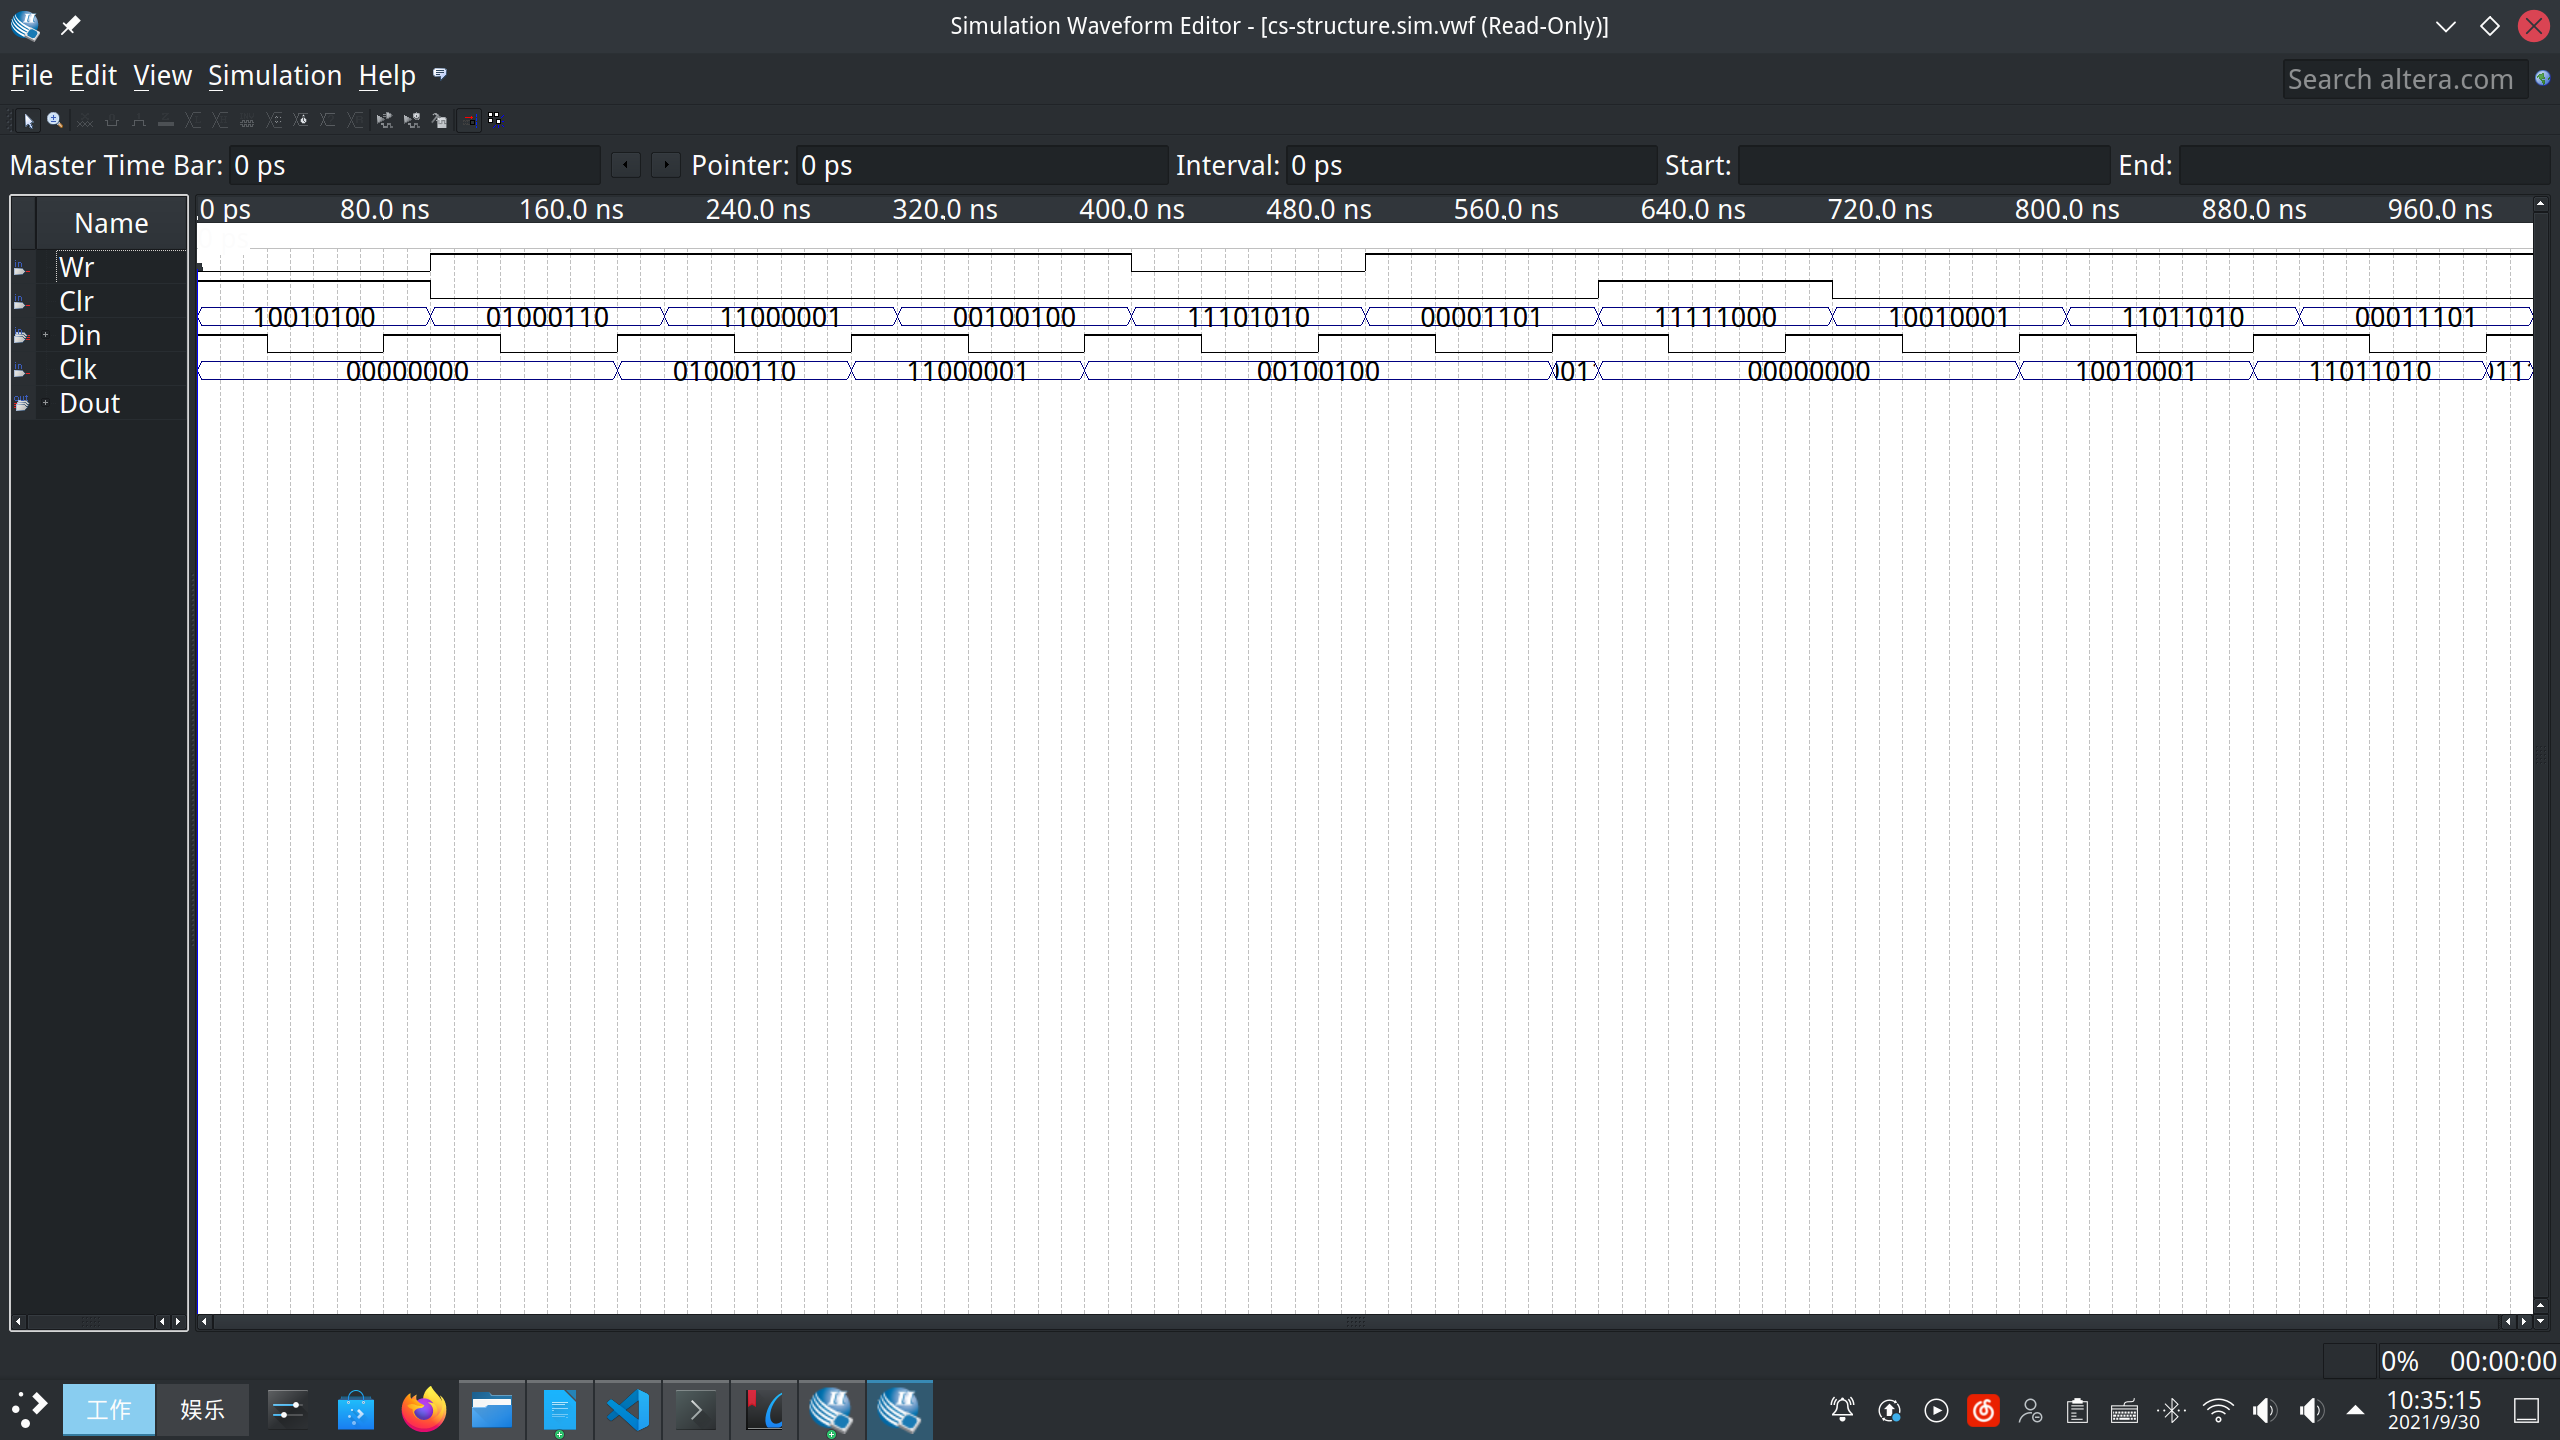
\includegraphics[scale=0.2]{pics/1.1-result.png}
\end{figure}

结果表明,D 触发器的功能正常。

\subsection{设计寄存器组}

实验验证使用的输入波形与输出波形(部分)如图 \ref{figure:1.2-result} 所示。

\begin{figure}[h]
    \centering
    \caption{寄存器组验证结果}
    \label{figure:1.2-result}
    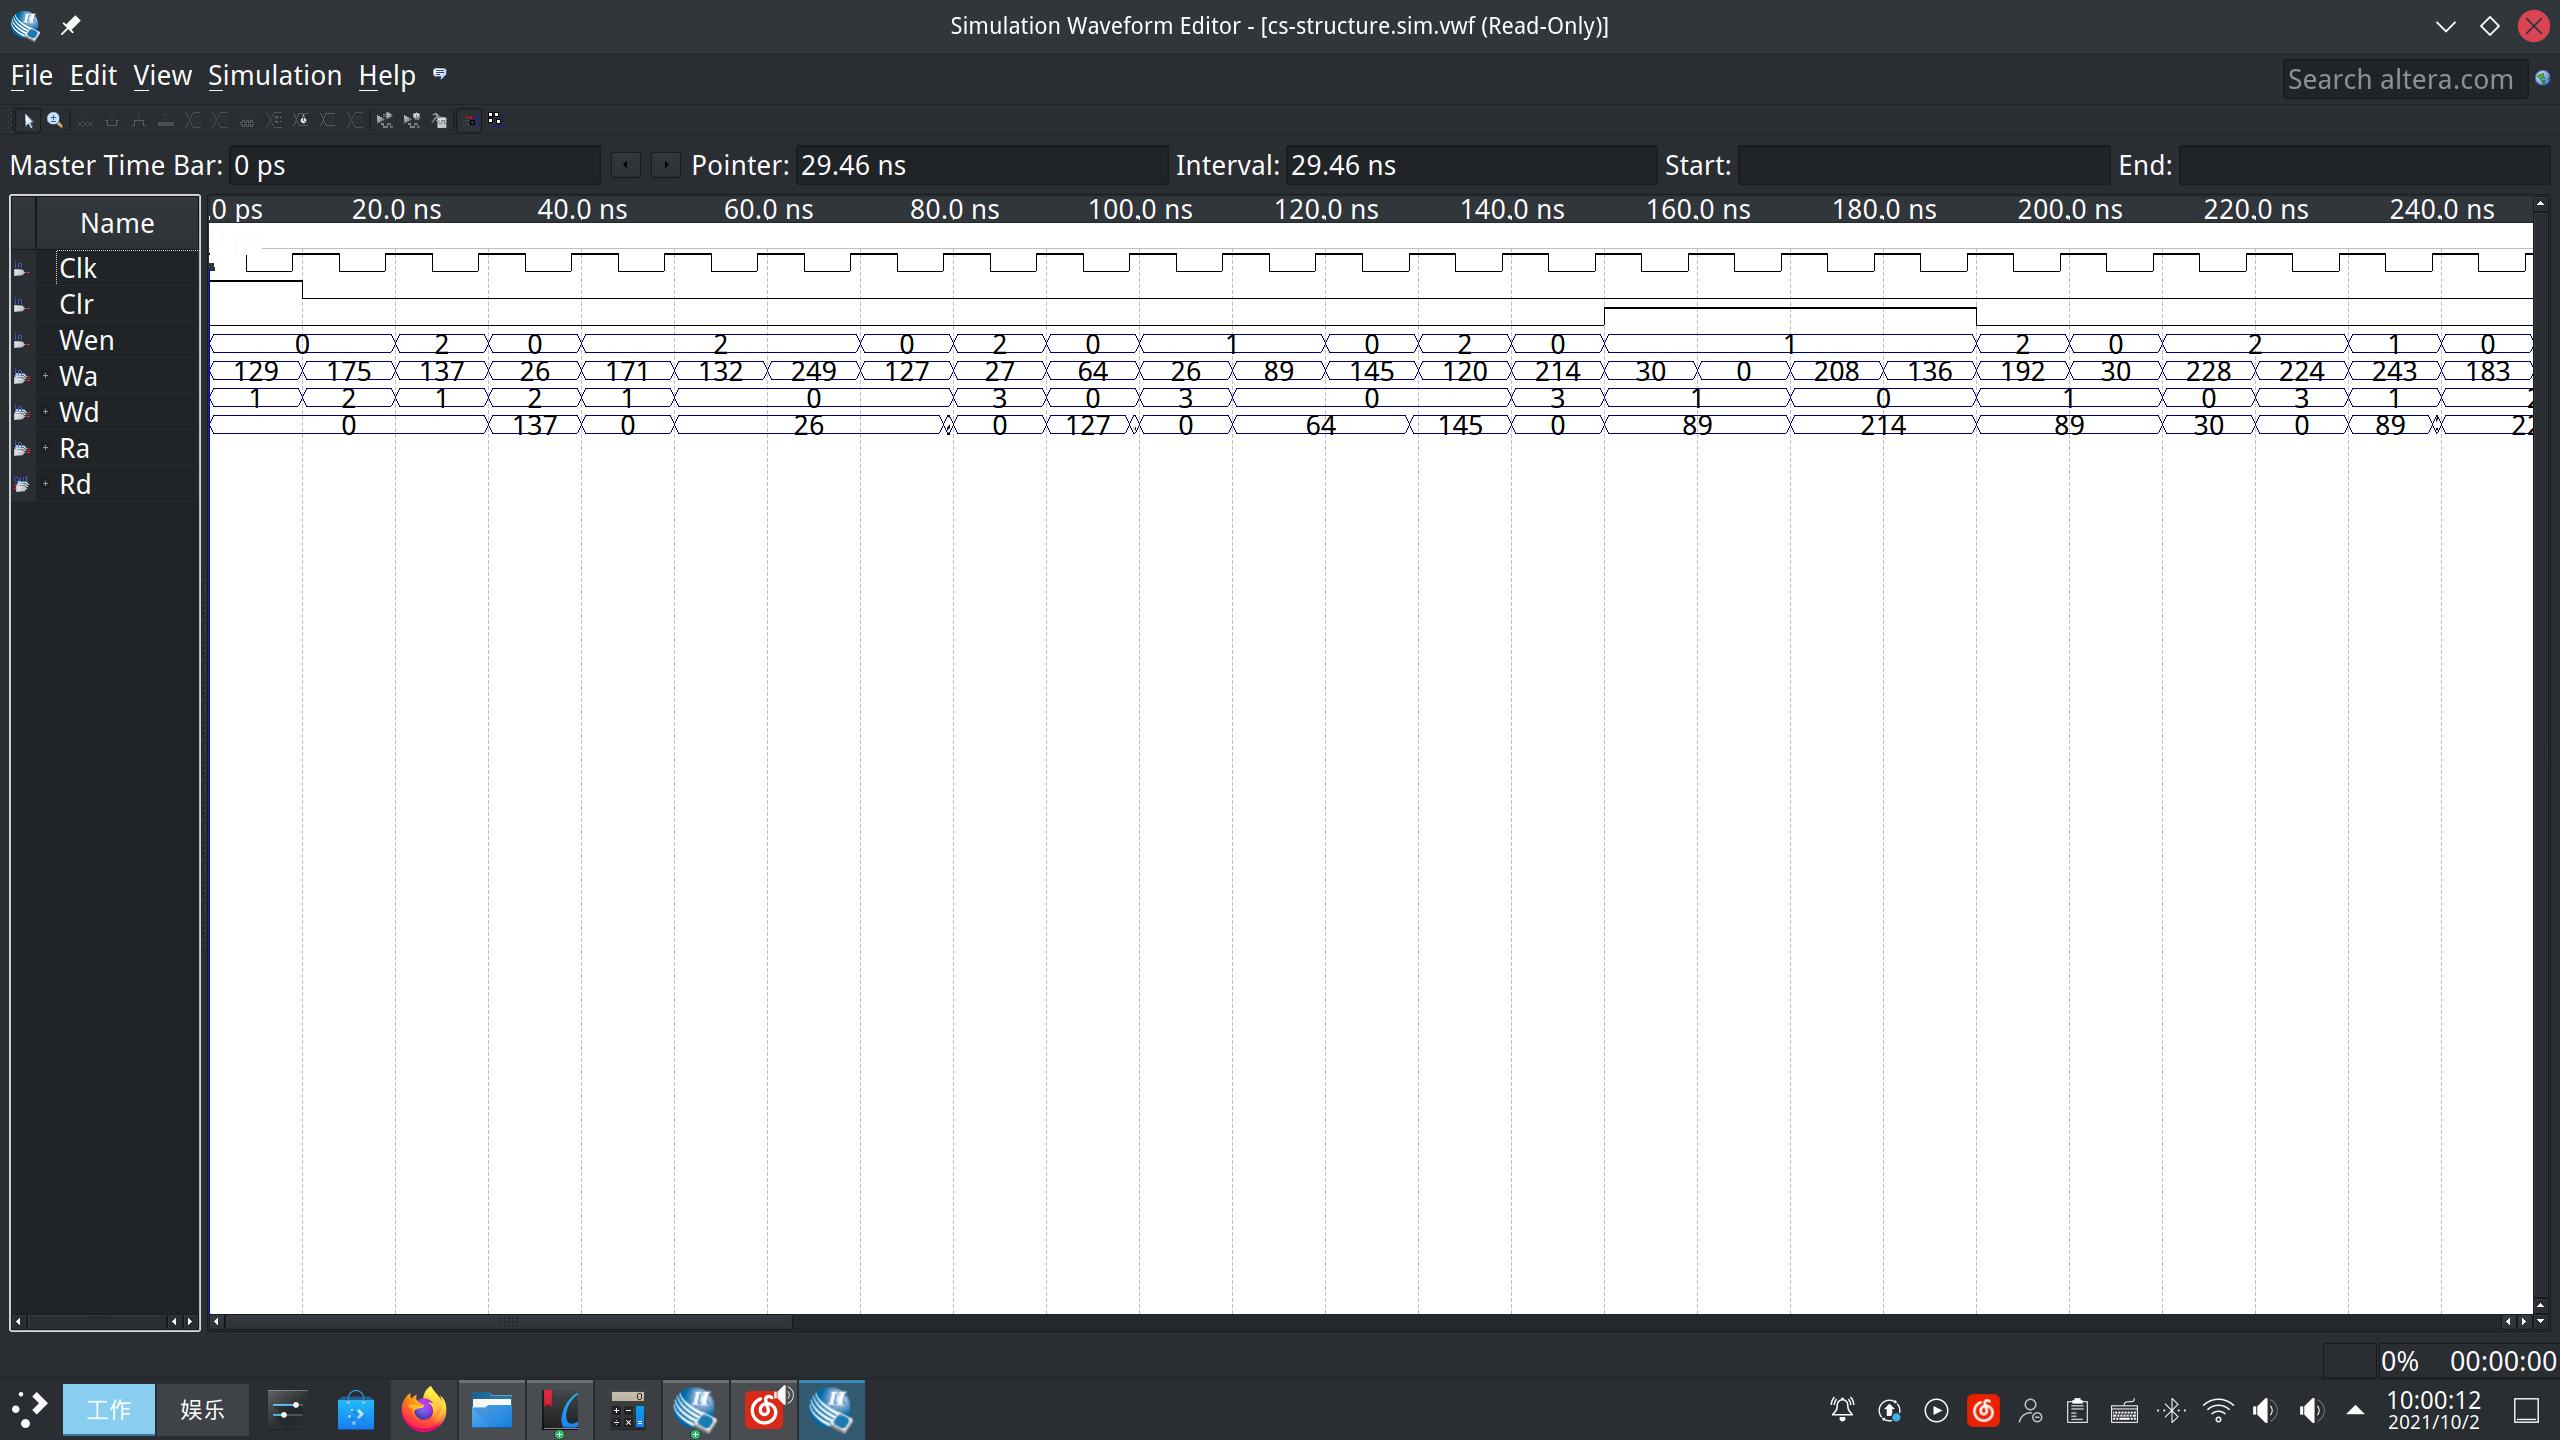
\includegraphics[scale=0.2]{pics/1.2-result.png}
\end{figure}

结果表明,设计的寄存器组功能正常。

\section{源文件列表}

见表 \ref{table:1-files}。

\begin{table}[h]
    \centering
    \caption{实验一源文件列表}
    \label{table:1-files}
    \begin{tabular}{|c|c|}
        \hline
        文件名称 & 说明 \\ \hline
        \verb|test_dff.bdf| & D 触发器功能验证设计图 \\ \hline
        \verb|test_lpm.vwf| & D 触发器功能验证波形图 \\ \hline
        \verb|test_4x8_storage.bdf| & $4 \times 8$ 寄存器组设计图 \\ \hline
        \verb|test_4x8_storage.vwf| & $4 \times 8$ 寄存器组验证波形图 \\ \hline
    \end{tabular}
\end{table}